\documentclass[titlepage=true]{scrartcl}

\input{header/zusammenfassung}
\input{header/hyperref}

\setDefaultArrayStretch{1.8}

\title{MikroelSys1}
\author{Jürg Rast}

\begin{document}
\begin{titlepage}
	\thispagestyle{empty}
	\maketitle
\end{titlepage}

\tableofcontents
\newpage

\section{CMOS Technologie\skript{Kap. 3}}

\section{Schaltungselemente in CMOS\skript{Kap. 4}}
Absolutwerte von Widerständen und Kapazitäten können um mehr als $\pm 20\%$ Abweichen! Viel genauer lassen sich Verhältnisse herstellen, dort sind Toleranzen von
unter $1\%$ üblich.

\subsection{Kapazitäten}
Es gibt im wesentlichen drei unterschiedliche Arten von Kapazitäten, welche in einem CMOS-Chip realisiert werden können: 
Poly-Poly-Kapazität ($C'' \approx 1fF/\mu m^2$),
MOS-Kapazität ($C'' \approx 10fF/\mu m^2$),
MIM-Kapazität (Metall-Isolator-Metall, $C'' \approx 1fF/\mu m^2$). $C''$ bezeichnet dabei die spezifische Kapazität pro Flächeneinheit.
Der Plattenabstand $d$ ist meist durch die Herstellung gegeben.

\begin{tabularx}{\linewidth}{|l|X|}
	\hline
	Elektrische Feldkonstante	& $\epsilon_0 = 8.85 \cdot 10^{-12} F/m$
	\\ \hline
	Kapazität/Fläche	& $C'' = \cfrac{\epsilon}{d} = \cfrac{\epsilon_0 \epsilon_r}{d}$
	\\ \hline
	Kapazität & $C = C'' \cdot A$
	\\ \hline
\end{tabularx}

\subsection{Widerstände}
Widerstände in CMOS sind meist unerwünscht da sie viel Platz brauchen und viel Wärme entsteht. Sollte trotzdem ein
Widerstand erforderlich sein, so lässt so ist er über seine Breite und Länge zu definieren:
\[
	R = R_\diamond \frac{L}{W}
\]

\begin{tabularx}{0.8\linewidth}{|l|l|X|l|l|}
	\hline
	\multicolumn{5}{|c|}{\textbf{Typische Werte für Widerstände}}
	\\ \hline
	Poly-Widerstand & $R \approx 10 \Omega/\diamond$ & & HR-Poly-Widerstand & $R \approx 1k\Omega/\diamond$
	\\ \hline
	P-Diffusions-Widerstand & $R \approx 100\Omega/\diamond$ & & N-Diffusions-Widerstand & $R \approx 100\Omega/\diamond$
	\\ \hline
	N-Well-Widerstand & $R \approx 1k\Omega/\diamond$ & & &
	\\ \hline
\end{tabularx}

\section{MOS-Transistoren\skript{Kap. 5}}

% \subsection{Allgemeine Begriffe und Formeln}
%TODO: was ist hier noch nötig?

\subsection{Bestimmung des Arbeitsbereichs}

\begin{enumerate}
	\item Bestimmung ob weak, moderate oder strong inversion.
	\item Berechnen der Sättigungsspannung.
	\item Wenn $V_{DS} > V_{DS,sat}$, $\Rightarrow$ gesättigt.
\end{enumerate}

\begin{tabular}{|l|l|l|}
	\hline
	\textbf{Arbeitsbereich}	& \textbf{Bedingung}					& \textbf{Sättigungspannung}
	\\ \hline
	weak inversion			& $0 < V_{GS} < V_T - 60mV$				& $V_{DS,sat} \approx 5\Phi_t \approx 130mV \quad \text{(bei } T = 300K \text{)}$ \\
	$I_D' < I_M'$			&										& $V_{GS} = V_{M} + h_{M} \cdot \Phi_t \cdot 																\ln{\frac{I_{D}}{\frac{W}{L} \cdot I_{M}}}$ 
	\\ \hline
	moderate inversion		& $V_T - 60mV < V_{GS} < V_T + 160mV$	& \\
	$I_M' < I_D' < I_H'$ 	& 										&
	\\ \hline
	strong inversion		& $V_T + 160mV < V_{GS} $				& $V_{DS,sat} = V_{GS} - V_T = \sqrt{\frac{{2 I_{D}}}{\beta}} = \sqrt{\frac{2 I_{D}}{\frac{W}{L} \cdot \beta_{0}}}$
	\\ 
	$I_H' < I_D'$ & & \\ \hline
\end{tabular} \\

mit $I_D = \frac{W}{L} I_D'$ \hspace{5mm} und \hspace{5mm} $\Phi_t = \frac{kT}{e}$, wobei $k = 1.38 \cdot 10^{-23} \frac{J}{K}$, und $e = 1.6 \cdot 10^{-19}C$ \\

\subsection{Kennlinien}
\subsubsection{Ausgangskennlinie}
\begin{minipage}{8cm}
	\centering
	\includegraphics[width=7cm]{images/Ausgangskennlinie.png}
\end{minipage}
\begin{minipage}{10cm}
	\textbf{Gesättigt}, Stromquellen-Betrieb:\\
	Geraden horizontal, dann ist $r_{DS}=\infty$ (idealer Transistor). \\
	Anstieg der Geraden entspricht Ausgangsleitwert $g_0$ bzw. Ausgangswiderstand $r_{DS}$. \\
	
	\textbf{Ungesättigt}, Widerstandsbetrieb: \\
	Je steiler die Gerade, desto kleiner $r_{DS}$. \\
\end{minipage}

\subsubsection{Transferkennlinie}
{	\centering
		\adjustbox{scale=0.7}{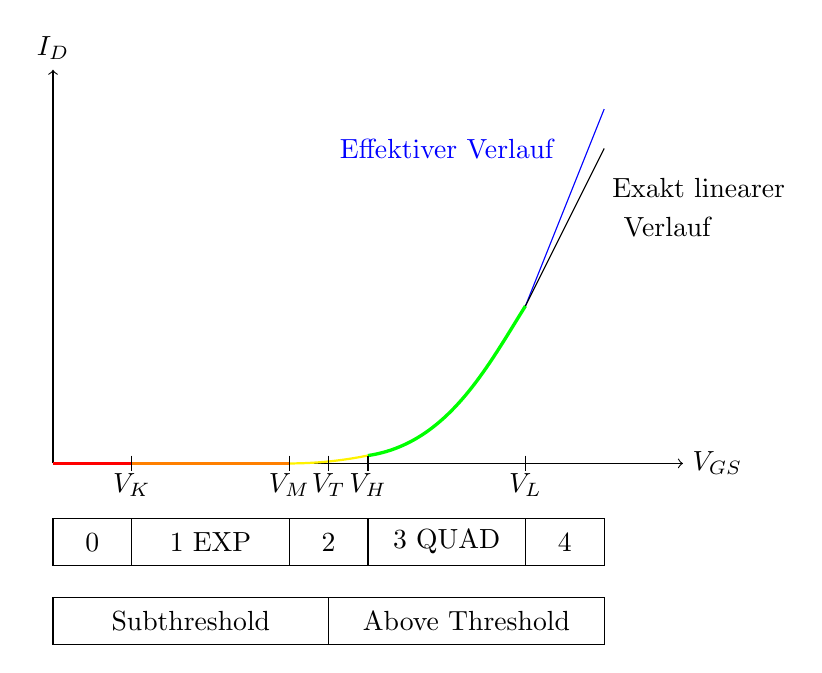
\begin{tikzpicture}

\draw [->] (0,0) -- (0,5) node [anchor=south] {$I_D$};
\draw [->] (0,0) -- (8,0) node [anchor=west] {$V_{GS}$};

\draw [color=red, thick] (0,0) -- (1,0);
\draw [color=orange, very thick] (1,0) -- (3,0);
\draw [color=yellow, thick] (3,0) arc (-90:-78:5);
\draw [color=green, very thick] (4.0,0.1) .. controls (5,0.25) and (5.5,1.2) .. (6,2);
\draw [color=blue] (6,2) -- (7,4.5);
\draw (6,2) -- (7,4);

\node [color=blue] at (5,4) {Effektiver Verlauf}; 
\node at (8.2,3.5) {Exakt linearer};
\node at (7.8,3) {Verlauf};


\foreach \x in {1,3,4,6} {
	\draw (\x,0.1) -- (\x,-0.1);
	\draw (\x,-0.7) -- (\x,-1.3);
}

\draw (3.5,0.1) -- (3.5,-0.1);

\draw (0,-0.7) rectangle (7,-1.3);

\node at (1,0) [anchor=north] {$V_K$};
\node at (3,0) [anchor=north] {$V_M$};
\node at (3.5,0) [anchor=north] {$V_T$};
\node at (4,0) [anchor=north] {$V_H$};
\node at (6,0) [anchor=north] {$V_L$};

\node at (0.5,-1) {0};
\node at (2,-1) {1 EXP};
\node at (3.5,-1) {2};
\node at (5,-1) {3 QUAD};
\node at (6.5,-1) {4};

\draw (0,-1.7) rectangle (7,-2.3);
\draw (3.5,-1.7) -- (3.5,-2.3);
\node at (1.75,-2) {Subthreshold};
\node at (3.5+1.75,-2) {Above Threshold};
\end{tikzpicture}}
	\qquad\qquad
		\includegraphics[width=7cm]{images/Transferkennlinie.png}
} \\

\setArrayStretch{1.1}
\begin{tabular}{|lp{3cm}|p{6cm}|p{8cm}|}
	\hline
	& \textbf{Ausgangs\-strom\-bereich} & \textbf{Mathematische Charakterisierung} & \textbf{Zugrundeliegender physikalischer Effekt}
	\\ \hline
	\cellcolor{red!70}
	0 
	& Leckstrombereich (LECK) 
	& $I_D$ erreicht Minimalwert, der nicht weiter unterschritten werden kann
	& Drain-Substratdiode und Source-Substratdiode haben Leckströme im Substrat
	\\ \hline
	\cellcolor{orange!70}
	1
	& Exponentieller Bereich (EXP)
	& $I_D$ steigt exponentiell mit $V_{GS}$
	& Kanal zeigt schwache Inversion (Beim n-Kanal-Transistor: Ursprünglich p-leitender Kanal ist schwach n-leitend)
	\\ \hline
	\cellcolor{yellow!70}
	2
	& Schwellen Bereich (MOD)
	& Keine "`handlichen"' Formel für $I_D$ vorhanden
	& Kanal zeigt moderate Inversion (Kanalzustand liegt zwischen schwacher und starker Inversion)
	\\ \hline
	\cellcolor{green!70}
	3
	& Quadratischer Bereich (QUAD)
	& $I_D$ steigt quadratisch mit $V_{GS}$
	& Kanal zeigt starke Inversion (Beim n-Kanal-Transistor: Ursprünglich p-leitender Kanal wirk stark n-leitend)
	\\ \hline
	\cellcolor{blue!70}
	4
	& Linearer Bereich (LIN)
	& $I_D$ steigt annähernd linear mit $V_{GS}$ (halb QUAD, halb LIN)
	& Geschwindigkeitsänderung der Ladungsträger im Kanal (die Ladungsträger können nicht weiter beschleunigt werden)
	\\ \hline
\end{tabular}
\resetArrayStretch


\subsection{Drainstromgleichungen}
\setArrayStretch{1.4}
\begin{tabular}{|p{3.8cm}|l|l|}
	\hline
		\textbf{Ausgangsstrom} 
		& \multicolumn{2}{c|}{\textbf{Ausgangsspannungsbereich} ($V_{DS}$-Bereich)}
	\\
		($I_D-, V_{GS}$-Bereich)
		& Transistor ungesättigt ($|V_{DS}| < |V_{DS,sat}|$)
		& Transistor gesättigt ($|V_{DS}| > |V_{DS,sat}|$)
	\\ \hline
		\multicolumn{3}{|c|}{\textbf{n-Kanal Transistor}}
	\\ \hline
		EXP-Bereich \newline (weak inversion)
		& $I_D = I_M e^{\frac{V_{GS}-V_M}{n_M \Phi_t}} (1-e^{\frac{-V_{DS}}{\Phi_t}}) (1 + \lambda V_{DS})$
		& $I_D = I_M e^{\frac{V_{GS}-V_M}{n_M \Phi_t}} (1 + \lambda V_{DS})$
	\\ \hline
		QUAD-Bereich \newline (strong inversion)
		& $I_D = B [(V_{GS} - V_T) V_{DS} - \frac{V_{DS}^2}{2}] (1 + \lambda V_{DS})$
		& $I_D = \frac{\beta}{2}(V_{GS} - V_T)^2 (1 + \lambda V_{DS})$
	\\ \hline
		\multicolumn{3}{|c|}{\textbf{p-Kanal Transistor}}
	\\ \hline
		EXP-Bereich \newline (weak inversion)
		& $I_D = I_M e^{-\frac{V_{GS}-V_M}{n_M \Phi_t}} (1-e^{\frac{-V_{DS}}{\Phi_t}}) (1 - \lambda V_{DS})$
		& $I_D = I_M e^{-\frac{V_{GS}-V_M}{n_M \Phi_t}} (1 - \lambda V_{DS})$
	\\ \hline
		QUAD-Bereich \newline (strong inversion)
		& $I_D = -B [(V_{GS} - V_T) V_{DS} - \frac{V_{DS}^2}{2}] (1 - \lambda V_{DS})$
		& $I_D = -\frac{\beta}{2}(V_{GS} - V_T)^2 (1 - \lambda V_{DS})$
	\\ \hline
\end{tabular} \\

Wird die Kanallängenmodulation vernachlässigt, kann einfach der $(1 - \lambda V_{DS})$ Term weggelassen werden. \\

\subsection{Kleinsignal-Ersatzschaltbild}
\begin{figure}[htbp]
        \centering
        \begin{subfigure}[b]{5cm}
                \centering
                \adjustbox{scale=0.7}{\begin{circuitikz}[american, european resistors]
	\draw (1.5,0) node[circ, name=G] {} node[right] {G};
	\draw (4,0) node[circ, name=D] {} node[right] {D};
	\draw (4,-2) node[circ, name=S] {} node[right] {S};
	\draw (0,-2) -- (S);
	\draw (G) -- +(-1.5,0);
	\draw (3,0) to[R=$r_{DS0}$] +(0,-2);
	\draw (0,-2) to[V] ++(0,2) ;
	\draw (0,-2) -- + (0,-0.2) node[ground] {};
	\draw (D) -- +(-1,0);
	\draw[->, thick] (-0.9, -0.2) -- +(0,-1.4) node[midway, left] {$V_{GS}$};
\end{circuitikz}}
                \caption{Widerstandsbetrieb}
        \end{subfigure} \qquad \qquad
        \begin{subfigure}[b]{5cm}
                \centering
                \adjustbox{scale=0.7}{\begin{circuitikz}[american, european resistors]
	\draw (1.5,0) node[circ, name=G] {} node[right] {G};
	\draw (5,0) node[circ, name=D] {} node[right] {D};
	\draw (5,-2) node[circ, name=S] {} node[right] {S};
	\draw (0,-2) -- (S);
	\draw (G) -- +(-1.5,0);
	\draw (4,0) to[R=$r_{DS}$] +(0,-2);
	\draw (3,0) to[I,mirror,l=$g_mV_{GS}$] +(0,-2);
	\draw (0,-2) to[V] ++(0,2) ;
	\draw (0,-2) -- + (0,-0.2) node[ground] {};
	\draw (D) -- ++(-1,0) to[short, i_=$I_D$] +(-1,0);
	\draw[->, thick] (-0.9, -0.2) -- +(0,-1.4) node[midway, left] {$V_{GS}$};
\end{circuitikz}}
                \caption{Stromquellenbetrieb, PI-ESB}
        \end{subfigure} \qquad \qquad
        \begin{subfigure}[b]{5cm}
                \centering
                \adjustbox{scale=0.7}{\begin{circuitikz}[american, european resistors]
	\draw (1.5,0) node[circ, name=G] {} node[above] {G};
	\draw (5,2) node[circ, name=D] {} node[right] {D};
	\draw (5,-2) node[circ, name=S] {} node[right] {S};

	\draw (G) -- +(-1.5,0);
	
	\draw (G)  -- (3,0);
	\draw (3,2) to[I,mirror,l=$g_mV_{GS}$] (3,0);
	\draw (3,2) -- (D);
	
	\draw (3,0) to[R={$R_s$},mirror] +(0,-2);
	\draw (0,-2) to[V] ++(0,2) ;
	\draw (0,-2) -- + (0,-0.2) node[ground] {};
	\draw (S) -- (0,-2);
	\draw[->, thick] (-0.9, -0.2) -- +(0,-1.4) node[midway, left] {$V_{GS}$};
	
	\draw (4.2,2) to[R=$r_{DS}$,mirror] (4.2,-2);
	
\end{circuitikz}}
                \caption{Stromquellenbetrieb, T-ESB}
        \end{subfigure}        
\end{figure}
\subsection{Kleinsignalparameter}
\begin{tabularx}{\linewidth}{|X|l|l|}
	\hline
		& \textbf{Transistor ungesättigt} & \textbf{Transistor gesättigt} 
	\\ \hline
		& Kanalwiderstand bei $V_{DS}=0$:
		& Kanalwiderstand:
	\\
		& $r_{DS0} = \frac{dV_{DS}}{dI_D}|_{V_{DS}=0} = \frac{\Phi_t}{I_{D0}}$
		& $r_{DS} = \frac{dV_{DS}}{dI_D} = \frac{V_A + V_{DS}}{I_D} \approx \frac{V_A}{I_D}$
	\\ weak
		& Kanalwiderstand bei $V_{DS} = 0V \dots V_{DS,sat}$:
		& 
	\\ inversion
		& $r_{DS} = \frac{dV_{DS}}{dI_D} \approx \frac{\Phi_t}{I_D} e^{\frac{V_{DS}}{\Phi_t}}$ (ungenau, kaum benötigt)
		&
	\\ \cline{2-3}
		& $g_m$ nicht benötigt
		& Steilheit
	\\
		& 
		& $g_m =  \frac{dI_D}{V_{GS}} = \frac{I_D}{n_m \Phi_t}$	
	\\ \hline
		& Kanalwiderstand bei $V_{DS}=0$:
		& Kanalwiderstand:
	\\
		& $r_{DS0} = \frac{dV_{DS}}{dI_D}|_{V_{DS}=0} = \frac{1}{\beta (V_{GS} - V_T) (1 + \lambda V_{DS})}$
		& $r_{DS} = \frac{dV_{DS}}{dI_D} = \frac{V_A + V_{DS}}{I_D} \approx \frac{V_A}{I_D}$
	\\ strong
		& Kanalwiderstand bei $V_{DS} = 0V \dots V_{DS,sat}$:
		& $r_{DS} = \frac{dV_{DS}}{dI_D}|_{V_{DS}=0} = \frac{1}{\beta [(V_{GS} - V_T)-V_{DS}] (1 + \lambda V_{DS})}$
	\\ \cline{2-3} inversion
		& $g_m$ nicht benötigt
		& Steilheit (zwei Formeln)
	\\
		&
		& $g_m = \frac{dI_D}{V_{GS}} = \beta (V_{GS} - V_T) (1 + \lambda V_{DS})$
	\\
		&
		& $g_m = \frac{dI_D}{V_{GS}} = \sqrt{2 I_D \beta (1 + \lambda V_{DS})} $
	\\ \hline
\end{tabularx}

\subsection{Parameter}

\begin{longtable}{|l|l|p{11cm}|}
	\hline
		$V_{DS,sat}$	& Sättigungsspannung	&
	\\ \hline
		$a_A$			& Early-Faktor			&
	\\ \hline
		$V_T$ & Schwellenspannung &
		Typisch $0.6V$ beim n-Kanal, resp. $-0.6V$ beim p-Kanal. $V_T$ ist stark von der Source-Bulk-Spannung abhängig (Body-Effekt):
		\[ 
			V_T = V_{T0} \pm \Delta V_T \quad \text{mit} \quad \Delta V_T = \gamma(\sqrt{V_{SB} \pm \Phi_0} -\sqrt{\Phi_0})
		\]
		positives Vorzeichen für n-Kanal, negatives für p-Kanal, $\gamma_N \approx 0.6\sqrt{V}$, $\gamma_P \approx 0.5\sqrt{V}$, $\Phi_{0} = 0.6V$ 
	\\ \hline
		$\Phi_t$ & Temperaturspannung &
		\[
			\Phi_t = V_{Temp} = \frac{kT}{e} = 86.2 \frac{\mu V}{K}T
		\]
		somit ist $\Phi_t = 25.9mV$ bei $T=300^\circ K$ bzw. $27^\circ C$
	\\ \hline
		$I_M$ & Drainstrom &
		Drainstrom an der Grenze zwischen schwacher und moderater Inversion.
		\[
			I_M = \frac{W}{L} \cdot I_M'
		\]
		$I_M'$ ist der spezifische Drainstrom an der Grenze
	\\ \hline
		$n_M$ & Unterschwellen-Neigungsfaktor &
		Der Faktor $n_m$ ist von der Source-Bulk-Spannung $V_{SB}$ abhängig:
		\[
			n_M = 1 + \frac{\gamma}{2 \sqrt{V_{SB} + \Phi_0}}
		\]
		mit $\Phi_0 = 2 \Phi_F \approx 0.6V$. 
		Für $V_{SB} = 0$ erhalten wir $n_M=1.39$. Häufig wird ein Wert von $n_M \approx 1.5$ angegeben.
	\\ \hline
		$V_A$			& Early-Spannung		& $V_A \approx a_A \cdot L$ \quad $V_{A}$ ist immer positiv
	\\ \hline
		$\lambda$ & Kanallängen-Modulationsfaktor &
		inverser Wert der Early-Spannung
		\[
			\lambda = \frac{1}{V_A} \approx \frac{1}{a_A L}
		\]
		Der MOS-Transistor wird vielfach mit $\lambda = 0$ idealisiert, was die Handrechnung vereinfacht.
	\\ \hline
		$B, \beta$ & Transkondukdanz &
		Steilheit, Verstärkungsfaktor. Dieser Faktor ist im gesättigten und ungesättigten Betrieb \textbf{grundsätzlich verschieden}. Es gilt: $\beta = \frac{W}{L} \beta_0 = \frac{W}{L} \mu C_{ox}''$. 
	\\ \hline
		$g_{m}$	& Transkonduktanz & Steilheit oder Gate-Steilheit. Beschreibt Zusammenhang zwischen $I_{DS}$ und $V_{GS}$. Mass für die Verstärkung.
	\\ \hline
		$g_{mb}$ & Body-Transkonduktanz & Beschreibt Wirkung des Body-Effekts. Nur im gesättigtem Stromquellenbetrieb von Bedeutung. Berechnung siehe Zbinden Formeln.
	\\ \hline
		$g_{0}$ & Ausgangsleitwert &
	\\ \hline
		$r_{DS}$ & Ausgangswiderstand & $r_{DS} = \frac{1}{g_0} \approx \frac{\Delta 	V_{DS}}{\Delta I_D} \quad 
													  \text{oder} \quad r_{DS} = \frac{V_A + V_{DS}}{I_{D,real}} \approx \frac{V_A}{I_D} $ 
	\\				&			&$V_{A}, V_{DS}, I_{D,real}$ immer im Betrag  
	\\ \hline
		$r_{s}$	& innerer Source-Widerstand & $r_{s} = \frac{1}{g_{m}}$
	\\ \hline
\end{longtable}


\section{Grundschaltungen mit MOS-Transistoren}

\section{MOS-Diode}

\section{MOS-Transistor als Stromquelle}

\section{MOS Stromspiegel\skript{Kap. 9}}
Ziel: Aus einer einzelnen genauen Strom- oder Spannungsquelle verschiedene genaue Ströme erzeugen.

\begin{tabularx}{\linewidth}{|l|l|X|}
	\hline
	Stromspiegelverhältnis & $n_m$ & $n_m = \frac{I_0}{I_i} = \frac{(\frac{W}{L})_{out}}{(\frac{W}{L})_{in}} \approx \frac{i_0}{i_i}$
	\\ \hline
\end{tabularx}

\subsection{Die wichtigsten Formeln}
\begin{multicols}{2}
	\textbf{Stromspiegelverhältnis}
	\[
		n_m = \frac{I_o}{I_i} 
			= \frac{\left(\frac{W}{L}\right)_o}{\left(\frac{W}{L}\right)_i}
			= \frac{I_{Do}}{I_{Di}}
	\]
	\columnbreak
		
	\textbf{Berechnung Ausgangsstrom}
	\[
		I_{out} = I_{in}\cdot\frac{W_{T_{out}}}{W_{T_{in}}}
	\]
	gilt nur wenn $L_{T_{out}} = L_{T_{in}}$
\end{multicols}


\begin{tabular}{|l|c|l|l|l|}
	\hline
	\textbf{Stromspiegeltyp} & \textbf{Genauigkeit} & \boldmath{$r_{out}$} & \boldmath{$V_I$} & \boldmath{$V_{O,min}$}
	\\ \hline
	Widlar Stromspiegel		& $+$	& $= \frac{1}{g_0}$								& $\approx V_T + \sqrt{\frac{2I_I}{\beta}}$		& $\approx \sqrt{\frac{2I_0}{\beta}}$
	\\ \hline
	Wilson Stromspiegel		& $+$	& $\approx \frac{1}{g_0}(2 + \frac{g_m}{g_0})$	& $\approx 2V_T + 2\sqrt{\frac{2I_I}{\beta}}$	& $\approx V_T + 2\sqrt{\frac{2I_0}{\beta}}$
	\\ \hline
	Verbesserter Wilson		& $++$	& $\approx \frac{1}{g_0}(2 + \frac{g_m}{g_0})$	& $\approx 2V_T + 2\sqrt{\frac{2I_I}{\beta}}$	& $\approx V_T + 2\sqrt{\frac{2I_0}{\beta}}$
	\\ \hline
	Kaskode-Stromspiegel	& $++$	& $\approx \frac{1}{g_0}(2 + \frac{g_m}{g_0})$	& $\approx 2V_T + 2\sqrt{\frac{2I_I}{\beta}}$	& $\approx V_T + 2\sqrt{\frac{2I_0}{\beta}}$
	\\ \hline
	geregelte Kaskode		& $++$	& $\approx \frac{1}{g_0}(\frac{g_m}{g_0})^2$	& $\approx V_T + \sqrt{\frac{2I_I}{\beta}}$		& $\approx 2\sqrt{\frac{2I_0}{\beta}}$
	\\ \hline
\end{tabular}



\begin{figure}[h]
	\centering
	\begin{subfigure}[b]{3cm}
		\centering
		{\includegraphics[width=3cm]{images/stromspiegel/widlar.png}}
		\caption{Widlar}
	\end{subfigure} \qquad	
	\begin{subfigure}[b]{3cm}
		\centering
		{\includegraphics[width=3cm]{images/stromspiegel/wilson.png}}
		\caption{Wilson}
	\end{subfigure} \qquad	
	\begin{subfigure}[b]{3cm}
		\centering
		{\includegraphics[width=3cm]{images/stromspiegel/verbesserter_wilson.png}}
		\caption{Verbesserter Wilson}
	\end{subfigure} \qquad	
	\begin{subfigure}[b]{3cm}
		\centering
		{\includegraphics[width=3cm]{images/stromspiegel/kaskode.png}}
		\caption{Kaskode}
	\end{subfigure} \qquad	
	\begin{subfigure}[b]{3cm}
		\centering
		{\includegraphics[width=3cm]{images/stromspiegel/geregelte_kaskode.png}}
		\caption{Geregelte Kaskode}
	\end{subfigure} 
	
	

	\caption{Die Stromspiegeltypen}
\end{figure}

\section{Einstufige MOS Verstärker}

\section{Frequenzverhalten von MOS Verstärker}

\section{MOS Operationsverstärker}

\section{Stabilität von MOS Operationsverstärker}

\section{Gebräuchliche Realisierungen von OTA's}

\section{Spannungsreferenzen}
\end{document}
